\documentclass[a4paper, 12pt]{article}

%packages
%\usepackage[dutch]{babel}
\usepackage{graphicx,subfigure}
\usepackage{amsmath,amsfonts,amsthm,amssymb}
\usepackage[margin=2cm]{geometry}
\usepackage{color}
\usepackage{shadethm}
%hyperlinks in document
\usepackage[bookmarks,colorlinks,breaklinks,linkcolor=blue]{hyperref}  % PDF hyperlinks, with coloured links
\usepackage{fancybox}

%\usepackage[T1]{fontenc}
%\usepackage{fontspec,xltxtra,xunicode}
%\defaultfontfeatures{Mapping=tex-text}
%\setromanfont[Mapping=tex-text]{Adobe Caslon Pro}
%\setsansfont[Scale=MatchLowercase,Mapping=tex-text]{Gill Sans}
%\setmonofont[Scale=MatchLowercase]{Andale Mono}

\newcommand{\boxtekst}[1]{%
  \fbox{%
      \addtolength{\linewidth}{-2\fboxsep}%
      \addtolength{\linewidth}{-2\fboxrule}%
      \begin{minipage}{\linewidth}%
     	#1 %
      \end{minipage}%
    }%
}

\renewcommand{\qedsymbol}{\hspace{\stretch{1}}\rule{1ex}{1ex} }
\newcommand{\ggd}{\ensuremath{\ \textrm{ggd}}}
\newcommand{\qdiv}{\ensuremath{\ \textrm{div} \ }}
\newcommand{\qmod}{\ensuremath{\ \textrm{mod} \ }}
\newcommand{\puntje}[1]{\ensuremath{ \Ovalbox{#1} }}
\newcommand{\etal}{\emph{et al.}}
\newcommand{\Angstrom}{\AA}
\newcommand{\degree}{^{\circ}}

\setlength{\parskip}{1.2em}
\setlength{\parindent}{0em}

% line spacing:
\usepackage{setspace} 
\setstretch{1.15}

\title{A Molecular Dynamics Model for DNA Hairpin Formation}
\author{Roald Frederickx \and Thomas in't Veld}
\date{May 2012}

\begin{document}

\maketitle

\begin{abstract}
We use a coarse-grained (three beads per nucleotide) molecular dynamics model of DNA to simulate the behaviour of DNA hairpin zipping and unzipping. In particular, we will examine the scaling of the zipping/unzipping time of a DNA hairpin with varying stem length $S$ and loop length $L$. Previous models that are based on a simple thermodynamic `zipper' predict a scaling of the unzipping time $\tau \sim S$ and an anomalous scaling of the zipping time of $\tau \sim S^{1.4}$. However, the model we will use also takes into account the inherent twisting of the stem that has to occur due to the helical nature of double stranded DNA (dsDNA). It has been shown via a simplified model that such twisting gives rise to a nontrivial scaling law for denaturation of dsDNA ($\tau \sim N^{2.6}$). We thus expect that, at least for the hairpin unzipping, we will find a deviation from the $\tau \sim S$ scaling law found with the simpler model. This finding is a valuable prediction for experimentalists as, to the best of our knowledge, there are no experimental results available to date concerning the stem length scaling law of DNA hairpin formation.
\end{abstract}

\tableofcontents

\section{Introduction}


Recent advances in nano- and biotechnology have brought a great deal of interest to the dynamics and structure of polynucleotides such as DNA. To understand the complex properties (such as self-assemblance), a good model of DNA is essential. The inherently large complexity of DNA molecules and their interactions, however, renders it difficult to find a simple theoretical model that is able to encompass all observed phenomena and complex behaviour of DNA. This is where computer simulations come in.\footnote{A review of current numerical simulation methods can be found in Slater \etal \cite{slater2009modeling} For a review of molecular dynamics methods for biophysics, see Karplus \& McCammon \cite{karplus2002molecular} and a recent overview specifically regarding molecular dynamics simulations of DNA can be found in P\'erez \etal\cite{perez2011frontiers}}

Depending on the behaviour that one tries to simulate, different levels of detail are needed. To investigate the smallest phenomena, a simulation of all the atoms in the molecule (and possibly the solvent) is needed. This is for instance the case when one wants to examine the precise role of active sites in enzymes \cite{weiner1986all}.  However, such simulations are computationally extremely expensive to run. For example, the microsecond simulation time barrier has only recently been broken, and that was for a dsDNA of only 12 nucleotides \cite{perez2007dynamics}.

To investigate macroscopical quantities, it often suffices to use a very coarse model of the actual DNA where lots of monomers are combined into a single entity. For instance, a popular model is that of a (self avoiding) random walk. Simulating such coarse-grained models is computationally cheap and can be done for very long timescales \cite{elber2005long}.

Concerning `coarseness', the model we use will be somewhere in between. It uses the three-sites-per-nucleotide approach due to Knotts, Rathore, Schwartz \& De Pablo \cite{knotts2007coarse} (called the 3SPN.0 model). It reduces the complexity of a nucleotide to three interaction sites (sugar, base, phosphate). The parametrization of that model was done by fitting it to experimental data of DNA-melting behaviour between 260--400\,K. An update to this model by the same group (Sambriski, Schwartz \& De Pablo \cite{sambriski2009mesoscale}) extends this model to also take into account the properties of the solvent (3SPN.1 model).

In 2011, Florescu \& Joyeux \cite{florescu2011thermal} further extended this model by slightly adjusting the interactions and contribution of the base pairing which gives better and more precise results for the denaturation of long DNA strands. This model (called the 3SPN.2 model from now on) thus gives a computationally cheap way of simulating the double helix structure of a DNA molecule, with experimentally fitted parameters that are available in the literature.



\subsubsection*{Goal}

We want to use this 3SPN model to research the effects of different loop structures (loop size, length of the complementary stem, \ldots) on interesting DNA behaviour, namely re/denaturation (`zipping/unzipping') and hairpin formation (the zipping of a single DNA strand with complementary base pairs, separated by a loop of non-complementary base pairs, as illustrated below).
\begin{verbatim}
                                                         X X
                                               --- CCTGCX   X
    ---CCTGCXXXXXXXXGCAGG---	      to           --- GGACGX   X
                                                         X X
\end{verbatim}We wrote a custom implementation of the 3SPN model with emphasis on performance, using the technique of spacial partitioning \cite{plimpton1995fast} to improve the performance of the (short ranged) nonbonded interactions.

The model will be used to investigate the scaling dynamics of the zipping and unzipping times of DNA hairpins with varying stem length. The formation of such hairpins in single stranded DNA has been shown to be very relevant for gene expression \cite{oettinger2000hairpins}. It has also been shown that hairpin formation is closely linked to translocation of DNA through nanopores \cite{carlon2011anomalous}. Hence, it is certainly relevant to have a better understanding of hairpin formation.

Previous simulations with a highly simplified Monte Carlo `zipper' model (Ferrantini \& Carlon \cite{carlon2011anomalous}) show a behaviour of the characteristic zipping time $\tau \sim S^{1.4}$ and an unzipping time $\tau \sim S$ with $S$ the stem length of the hairpin. However, that model did not take into account the inherent twisting of the stem that has to occur due to the helical nature of double stranded DNA.

The 3SPN model, however, will correctly represent these structural properties of a DNA hairpin and we will examine whether this changes the scaling behaviour. 

Simple models of DNA denaturation that take into account the helicity, predict scaling behaviour of the denaturation time of $\tau \sim N^{2.6}$ with $N$ the number of base pairs \cite{carlon2010unwinding}. 

Furthermore, because we will use a molecular dynamics simulation instead of a Monte Carlo algorithm, it will be possible to extract not only the scaling law, but also the actual pre-factors. These can be used to compare with experimental values to verify the correctness of the model. To the best of our knowledge, however, there is no experimental evidence to date that describes this scaling behaviour with varying stem length. Hence, the result of the model is a prediction.

On the other hand, the scaling with varying loop length (and composition) has received more experimental attention \cite{bonnet1998kinetics}. We will investigate the behaviour of 3SPN model in this regime as well, although we suspect that there will be deviations due to the coarseness of the model. We especially expect deviations for small loop sizes due to the hydrophobic interactions that are unaccounted for. Indeed, it is currently assumed \cite{vallone1999melting, shen2001loop} that these are responsible for deviations at small loop sizes. Nonetheless, it is interesting to see how the 3SPN model behaves in these circumstances, and how it compares to experiment.

In summery, we will use the 3SPN model to simulate a number of biophysical observables and processes that are not yet simulated with this model. We expect that the computational efficiency of the coarse grained model will be a significant advantage of the 3SPN model when simulating scaling behaviour, while still retaining a high degree of morphological accuracy.

\section{Methods}

Full atom simulations of DNA molecules exist (todo: citations) but are computationally very heavy. In 2007, the group of De Pablo \cite{knotts2007coarse} applied the technique of coarse graining to a molecular simulation of DNA: instead of simulating all atoms, a DNA monomer is represented by three sites: the sugar, the phosphate and the base. For simulations where one is mainly interested in the timescale behaviour or global dynamics of the DNA molecule this is a very good approximation: it is computationally cheap (and easy to optimize) while describing the DNA helical structure quite good. 

We implemented the 3SPN model with a few changes of our own. The codebase was not available publicly, so everything had to be created from scratch in C with an OpenGL rendering engine attached -- we decided to make it open source and available at GitHub: \href{https://github.com/RoaldFre/DNA}{github.com/RoaldFre/DNA}. The interested reader can find the full package containing everything needed to reproduce the material presented in this paper at that location.

\subsection{DNA structure}

In this paper, we follow the approach of Knotts, De Pablo \etal \cite{knotts2007coarse} to model the structure of B-DNA. In Figure \ref{dna_forms}, the main three structural forms of DNA are illustrated.

\begin{figure}[htbp]
\begin{center}
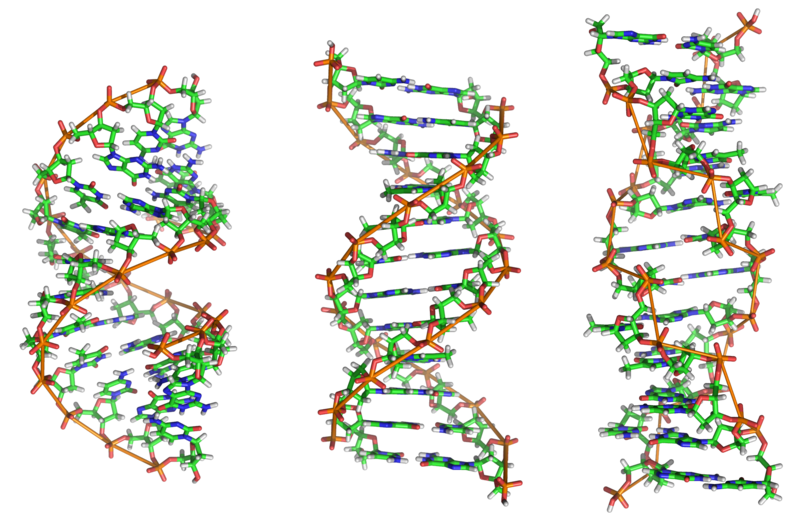
\includegraphics[width=14cm]{images/dna_forms.png}
\caption{Structural forms of DNA: A-DNA (left), B-DNA (center) and Z-DNA (right). Figure from \href{http://www.molecularstation.com}{molecularstation.com}.}
\label{dna_forms}
\end{center}
\end{figure}


The algorithm to build up a single strand is to follow the screw symmetry of B-DNA by placing consecutive monomers on the $z$-axis of space (separated by an axial rise of $3.38$\,\Angstrom), and rotating each consecutive monomer by an angle of $36$ degrees. In practice, this means that if a monomer is placed at location $(r, \phi, z)$, the consecutive monomer on the same strand is placed at $(r, \phi + 36\degree, z + 3.38\,\text{\Angstrom})$. To build up the complementary strand (yielding the characteristic double stranded helical structure of DNA), an atom at $(x, y, z)$ on the first strands has its complementary atom on the other strand at $(x, -y, -z)$ with the $x$-axis taken orthogonal to the helical axis and always along the line connecting the complementary bases of the complementary monomers (i.e. the $x$-axis also rotates $36\degree$ along the $z$-axis for consecutive base pairs along the double strand).

Knotts \etal \cite{knotts2007coarse} used the DNA molecular data of ref. \cite{crcBiochem1976}, and averaged positions for each of the three sites per nucleus yielding the data in table \ref{dnaStructureData}. Schematically, this structure yields the major and minor grooves as illustrated in Figure \ref{schematic_knotts}. The phosphate and sugar sites on the backbone of the molecule are placed at the centers of mass of the molecules; bases Ab and Gb are placed at the N1 position of the B-DNA isoform; bases Tb and Cb at the N3 position. 

\begin{table}[htdp]
\caption{Structural data for B-DNA helices, calculated by Knotts \etal \cite{knotts2007coarse}.}
\begin{center} \footnotesize
\begin{tabular}{|l|rrrrc|c|}
\hline
 &\ \  x (\Angstrom)\ \ &\ \  y (\Angstrom)\ \  &\ \  z (\Angstrom)\ \  &\ \  r (\Angstrom)\ \  &\ \  $\phi$ (degrees)\ \  & \ \ Mass (amu) \\
\hline
Phosphate (P) & -0.628 & 8.896 & 2.186 & 8.918 & 94.038 & 94.97 \\
Sugar (S) & 2.365 & 6.568 & 1.280 & 6.981 & 70.197 & 83.11 \\
Adenine base (Ab) & 0.575 & 0.516 & 0.051 & 0.773 & 41.905 & 134.1\\
Thymine base (Tb) & 0.159 & 2.344 & 0.191 & 2.349 & 86.119 & 125.1\\
Cytosine base (Cb) & 0.199 & 2.287 & 0.187 & 2.296 & 85.027 & 110.1\\
Guanine base (Gb) & 0.628 & 0.540 & 0.053 & 0.828 & 40.691 & 150.1\\
\hline
\end{tabular}
\end{center}
\label{dnaStructureData}
\end{table}%

In Figure \ref{methods_dnaStructure} two screenshots of our implemented model are given, showing a side view of the double helix structure and a top view of the internal structure of the bond and dihedral angles.

\begin{figure}[h]
\begin{center}
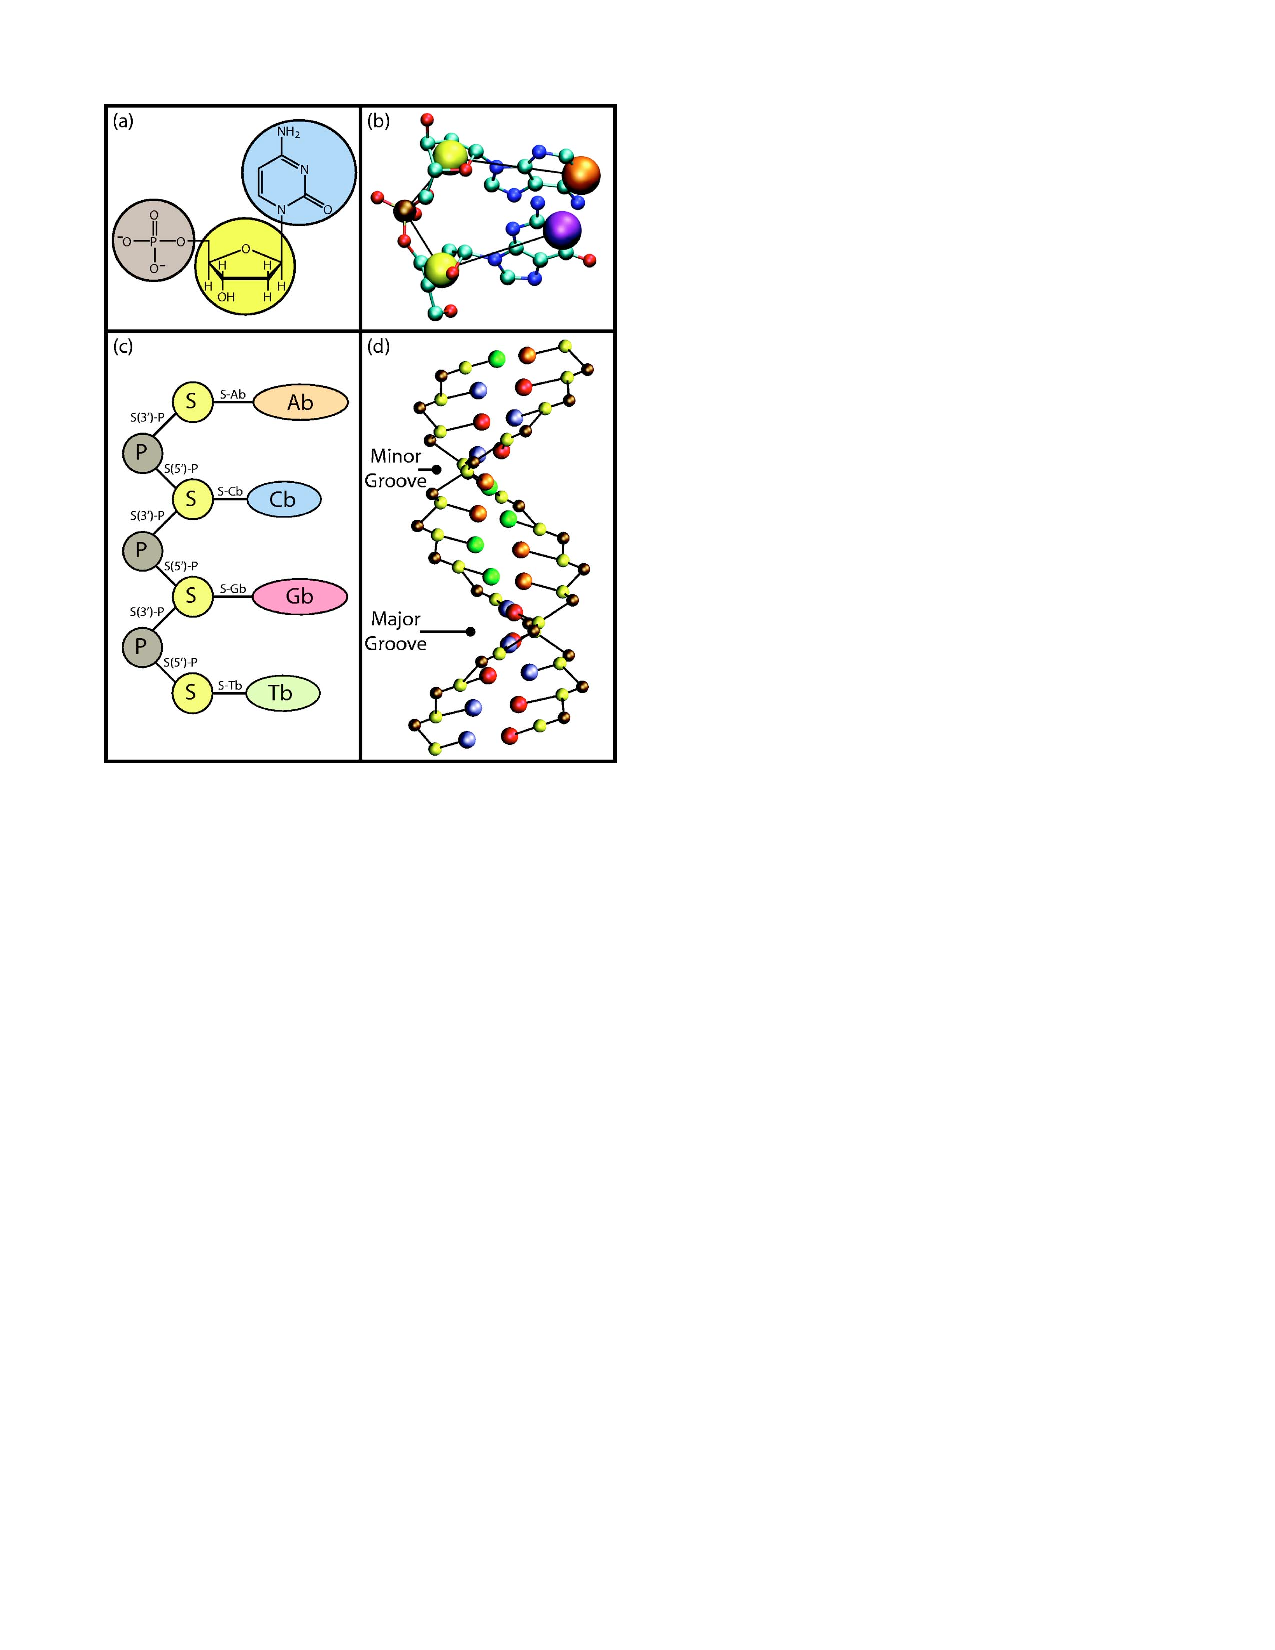
\includegraphics{images/schematic_structure_knotts}
\caption{The schematic structure of the model for B-DNA, from Knotts \etal \cite{knotts2007coarse}. Note the placing of the three sites per nucleus relative to the original atomic structure in the upper right panel.}
\label{schematic_knotts}
\end{center}
\end{figure}

\begin{figure}[h]
\begin{center}
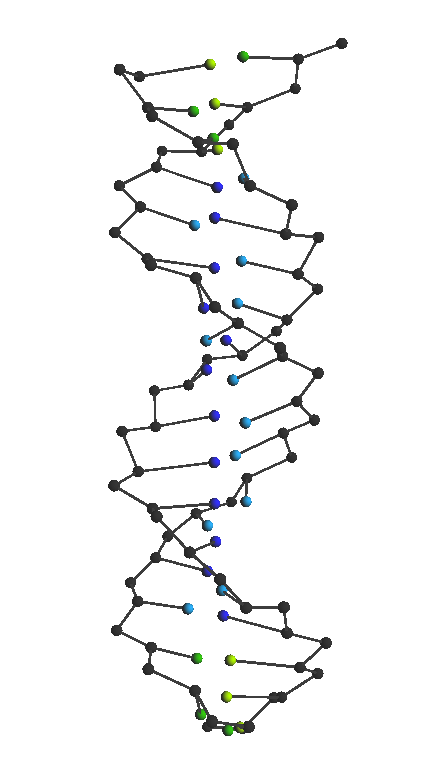
\includegraphics[width=5cm]{images/methods_dnaStructure1} 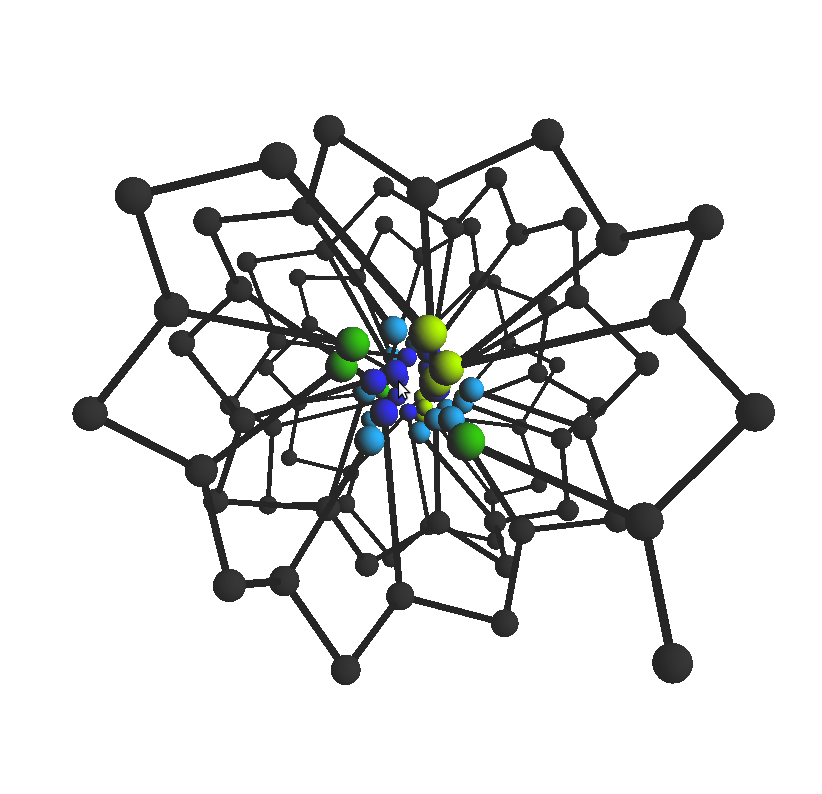
\includegraphics[width=7cm]{images/methods_dnaStructure2}

\end{center}\label{methods_dnaStructure}
\caption{Side- and top view of the dsDNA structure in our implemented model. The major and minor groove structure in the double helix is clearly visible; as is the screw symmetry from the top view.}
\end{figure}


\subsection{Interactions}

The potential energy of the complete system consists of
\begin{equation}
V_\text{total} = V_\text{bond} + V_\text{angle} + V_\text{dihedral} + V_\text{stack} + V_\text{bp} + V_\text{ex} + V_\text{qq}.
\end{equation}
The strengths of the individual iteractions will be expressed in terms of the energy unit $\varepsilon$, taken to be $0.26$\,kcal/mol. The potential energies are taken mainly from the potential terms as defined by Florescu \& Joyeux \cite{florescu2011thermal}, and are an improvement over the original terms by Knotts \etal \cite{knotts2007coarse}. However, in the end they are very much alike and interchangeable; and we opt for the conventions of the Florescu paper primarily because they are more clearly formulated. We will now sketch the specific potential energy terms one by one, but first we define a few constants regularly used in the potentials.

\begin{table}[hbt]\begin{center}
\begin{tabular}{llll}
Parameter & Value \qquad \qquad \qquad \qquad & Parameter & Value\\
\hline
$\varepsilon$ & $1.81\times10^{-21}$ Joule/particle\qquad\qquad & $k_\phi$ & $4\varepsilon$ \\
$k_1$ & $10^{20}\varepsilon$ in Joule/(\AA)$^2$ & $\varepsilon_\text{GC}$ & $16\varepsilon$\\

$k_2$ & $100\times10^{20}\varepsilon$ in Joule/(\AA)$^2$ & $\varepsilon_\text{AT}$ & $4\frac{2}{3} \varepsilon_\text{GC}$ \\
$k_\theta$ & $400\varepsilon$ per radian$^2$ & & \\
\end{tabular}
\caption{Regularly used energy constants for the potential energies, used by Knotts \etal \cite{knotts2007coarse}.}\end{center}
\end{table}

\paragraph{Bond potential} The typical expression for the intramolecular bonds between molecules in the same DNA strand is a sum over all bonds of a quadratic and a quartic potential term
\begin{equation}
V_{\text{bond}} = \sum_i^{N_{\text{bond}}} \left[ k_1 \left(d_i - d_{0_i}\right)^2 + k_2 \left(d_i - d_{0_i}\right)^4\right]
\end{equation}
(the `stretch' term) around equilibrium distances $d_{0_i}$ as defined in the standard B-form structure of double strand DNA, and coupling constants $k_1$ and $k_2$.

\paragraph{Bond angle potential} The angle that forms between three consecutively bound sites in a DNA strand is regulated by the sum over all bond angles of the quadratic term (`bend' force)
\begin{equation}
V_\text{angle} =  \sum_i^{N_\text{angle}} \frac{k_\theta}{2} \left( \theta_i - \theta_{0_i} \right)^2
\end{equation}
where we define an equilibrium angle $\theta_0$ from the DNA B-form, and a constant $K_\theta = 400\varepsilon / (\text{radian})^ 2$.

\paragraph{Dihedral angle potential} The third and last potential defining the structural properties of the strand regulates the dihedral angle between four consecutive bound sites on the same strand
\begin{equation}
V_\text{dihedral} =  \sum_i^{N_\text{dihedral}} k_\phi \left[ 1 - \cos (\phi_i - \phi_{0_i}) \right]
\end{equation}
with $\phi_{0_i}$ the equilibrium dihedral angle from the DNA B-form definitions, and constant $k_\phi = 4\varepsilon$.

\paragraph{Stacking potential} The stacking potential is a Leonard-Jones type potential describing the base stacking phenomena and regulates the rigidity of the DNA backbone,
\begin{equation}
V_\text{stack} =  \sum_{i<j}^{N_\text{stack}} \varepsilon \left[ \left(\frac{r^0_{ij}}{r_{ij}} \right)^{12} - 2\left(\frac{r^0_{ij}}{r_{ij}} \right)^{6} + 1\right]
\end{equation}
modeled with an effective cut-off distance of $9$\,\Angstrom because of over which . It is important to observe that this induces not only a stacking interaction between the $i$th and $(i+1)$th base, but also between the $i$th and $(i+2)$th base. (Hence the sum over all stackings $i$ and $j$, with $i < j$ to avoid double counting). $\sigma_{ij}$ depends on the type of bases for which the stacking is calculated.

\paragraph{Basepairing potential} A hydrogen bonding interaction between two complimentary bases (zero if not complementary) is written as
\begin{equation}
V_\text{bp} =  \sum_{\text{base pairs}}^{N_\text{bp}} \varepsilon_{\text{bp}_i} \left[ 5\left(\frac{r^0_{\text{bp}_i}}{r_{ij}} \right)^{12} - 6\left(\frac{r^0_{\text{bp}_i}}{r_{ij}} \right)^{10} + 1\right]
\end{equation}
where we have $r^0_{bp}$ depending on the type of complimentary basepair and coupling constants $\varepsilon_\text{GC}$ and $\varepsilon_\text{AT}$.

\paragraph{Exclusion potential} In the original and follow-up versions of the 3SPN model (Knotts \etal \cite{knotts2007coarse}, Sambriski \etal \cite{sambriski2009mesoscale}) a Leonard-Jones type potential was used to describe excluded volume interactions between mismatched bases (yielding $\sigma_0 = 1.0 \times 2^{-1/6}$\,\Angstrom) and other molecules (even on other strands) that do not interact via the Coulomb or basepairing potential (yielding $r_0 = 6.86 \times 2^{-1/6}$\,\Angstrom):
\begin{equation}
V_\text{excl} =  \sum_{i<j}^{N_\text{ex}}\begin{cases} 4\varepsilon \left[ \left(\frac{r_{0}}{r_{ij}} \right)^{12} - \left(\frac{r_{0}}{r_{ij}} \right)^{6} \right] + \varepsilon \qquad &\text{if }r_{ij} < d_\text{cut}, \\ 0 \qquad &\text{if }r_{ij} \geq d_\text{cut} \end{cases} \end{equation}
where a cut-off value of $d_\text{cut} = 5.86$\,\Angstrom\ is imposed. This will make sure two strands do not cross each other when simulating DNA hybridisation, and also that a single strand does not cross itself during a hairpin formation simulation. Florescu \& Joyeux \cite{florescu2011thermal} report that the exclusion potential is not necessary when simulating long double stranded DNA helices; we decided however to keep this potential for the above reasons. The cut-off value of $5.86$ \Angstrom\ we use, however, is a little bit smaller than the original value in Knotts and Sambriski \cite{knotts2007coarse, sambriski2009mesoscale} where $6.86$ \Angstrom\ is used; we find that by decreasing the cut-off value slightly we massively improve the (local) stability of the system without losing the crucial advantages of the exclusion potential.

\paragraph{Coulombic potential} The final potential in our model is the screened electrostatic Coulomb interaction between the phosphate molecules situated on the backbone of the DNA strands. It is modeled using a Debye-H\"uckel approximation with a Debye length $\kappa_D$ depending on the salt concentration of the environment,
\begin{equation}
V_\text{qq} =\sum_{i<j}^N  \frac{q_i q_j}{4\pi \varepsilon_0 \varepsilon_k r_{ij}} \exp \left(- \frac{r_{ij}}{k_D}  \right)
\label{coulomb}\end{equation}
where the Debye length can be written as
\begin{equation}
\kappa_D = \left( \frac{\varepsilon_0 \varepsilon_k RT}{2N^2_A e^2 I} \right)^{0.5}
\end{equation}
where we use the vacuum permittivity $\varepsilon_0$, Avogadro´s number $N_A$, the electronic charge $e$ and the ionic strength $I$. For the default value of the ionic strength [Na$^+$]=50 mM (milimolair, equal to milimol/liter) this yields $\kappa_D$ = 13.603\,\Angstrom. The other values in \ref{coulomb} are the dielectric constant $\varepsilon_k = 78$ for water, and the charges on the interacting molecules (phosphates, with $q_i = -1$ so $q_i q_j = 1$).

The interactions are defined so that two molecules are excluded from the nonbonded interactions if they constitute a bond. On top of that, $V_\text{stack}$, $V_\text{bp}$ and $V_\text{ex}$ are modeled as mutually exclusive. Our codebase makes sure that this is handled correctly, to avoid the unphysical pairing of bases on the same strand or to avoid cases where an exclusion potential is working on two sites already interacting via Coulombic interaction. All non-specified geometric and interaction constants are taken from Table III in \cite{knotts2007coarse}, which we reproduce in Table \ref{geometricConstants} for consistency's sake.

\begin{table}[htb]
\begin{tabular}{lccc}
\hline
Bond&$d_0$ (\AA)&Bond Angle& $\theta_0$ (degree) \\
\hline
S(5')-P & 3.899 & S(5')-P-(3')S & 94.49\\
S(3')-P & 3.559 & P-(5')S(3')-P & 120.15 \\
S-Ab & 6.430 & P-(5')S-Ab & 113.13\\
S-Tb & 4.880 & P-(3')S-Ab & 108.38\\
S-Cb & 4.921 & P-(5')S-Tb & 102.79\\
S-Gb & 6.392 & P-(3')S-Tb & 112.72\\
&&P-(5')S-Cb & 103.49\\
&& P-(3')S-Cb & 112.39\\
&& P-(5')S-Gb & 113.52\\
&& P-(3')S-Gb & 108.12\\
& & & \\
\hline
Dihedral Angle & $\phi_0$ (degree) & Nonbonded & Length (\AA) \\
\hline
P-(5')S(3')-P-(5')S & -154.80 & $r^0_{ij}$ & Interaction specific \\
S(3')-P-(5')S(3')-P & -179.17 & $r^0_{\text{bp}_\text{AT}}$ & 2.9002 \\
Ab-S(3')-P-(5')S & -22.60 & $r^0_{\text{bp}_\text{GC}}$ & 2.8694 \\
S(3')-P-(5')S-Ab & 50.69 & $r_0$ (mismatched bases) & $2^{-1/6} (1.0)$ \\
Tb-S(3')-P-(5')S & -33.42 & $r_0$ (otherwise) & $2^{-1/6} d_\text{cut}$ \\
S(3')-P-(5')S-Tb & 54.69 & & \\
Cb-S(3')-P-(5')S & -32.72 & $d_\text{cut}$ & $r^0 \approx 5.86$ \\
S(3')-P-(5')S-Cb	& 54.50 & & \\
Gb-S(3')-P-(5')S & -22.30 & & \\
S(3')-P-(5')S-Gb & 50.66 & & \\
\hline
\end{tabular}\label{geometricConstants}

\caption{Geometric constants for the potential energy functions as defined above. Important to note is that a sugar can bind to a phosphate in a 5' or a 3' sense; S(5')-P represents a sugar-phosphate bond inside the same nucleotide but S(3')-P is a bond between neighboring nucleotides. Bond angles like P-(5')S(3')-P include both kinds of bondings. The table is reproduced from Knotts \etal \cite{knotts2007coarse}.}
\end{table}

Because we work with a space partitioning scheme, we will also truncate the potential energies that we use at a certain chosen truncation length (default at $20$\,\Angstrom) and shift them so that they yield a potential energy of zero when calculated at the truncation distance.

\subsection{Space Partitioning}



\subsection{Dynamics}

\section{Results}
\section{Conclusions}

Time scaling behavior of hairpin formation by single stranded DNA structures was simulated with a coarse grained model modeling the DNA structure with three sites (base, sugar, phosphate) per nucleotide.

We found that the time scale of zipping of ssDNA hairpins behaves like
\begin{equation}
\tau_\text{zipping} \sim N^{\beta_z} \qquad \qquad \text{with}\ \beta_z = 1.2 \todo{!!!! final number!}
\end{equation}
in function of the stem length $N$, where other authors using more simple Monte Carlo based methods found time scaling with exponent $\beta_z = 1.37 \pm 0.02$. Our coarse grained molecular model thus confirms the earlier simulations of Ferrentini \& Carlon \cite{carlon2011anomalous}.

The unzipping of DNA hairpins is found in our model to have a timescale yielding
\begin{equation}
\tau_\text{unzipping} \sim N^{\beta_u} \qquad \qquad \text{with}\ \beta_u = 2.6,\todo{!!!! final number!}
\end{equation}
where previous simulations by Baiesi, Barkema, Carlon \& Panja \cite{carlon2010unwinding} and Baiesi \& Livi \cite{baiesi2009multiple} yielded ranges $\beta_u = 2.57(3) - 3$ with the first (and more recent) model having lower exponent values than the latter, more simple model. Our simulations thus confirm the scaling law with exponent $\beta_u \approx 2.6$ for hairpin unzipping.

We conclude that in the study of denaturation and renaturation of anomalous DNA structures like hairpins of ssDNA the effect of the twisted helix structure must be taken into account. We also conclude that the time scaling behavior indicated that DNA renaturation and denaturation are processes far from equilibrium.

Improvements to our methods certainly can be made. All simulations presented in this paper were done in the timeframe of less than one week -- it is inevitable that longer and more numerous simulations will yield better and more significant results (certainly concerning the error margins on the time scaling behavior that we found). Furthermore, we think that the model we implemented (although fast already) and the simulation scripts we used can be optimized further to attain more effici\"ent CPU time.



\footnotesize
\bibliographystyle{ieeetr}
	\bibliography{references}

\end{document}



